%!TEX TS-program = xelatex
% Исходная версия шаблона --- 
% https://www.writelatex.com/coursera/latex/5.1
\documentclass[c, dvipsnames]{beamer}  % [t], [c], или [b] --- вертикальное 
%\documentclass[handout, dvipsnames, c]{beamer} % Раздаточный материал (на слайдах всё сразу)
%выравнивание на слайдах (верх, центр, низ)
%\documentclass[handout, dvipsnames]{beamer} % Раздаточный материал (на слайдах всё сразу)
%\documentclass[aspectratio=169, dvipsnames]{beamer} % Соотношение сторон
\setbeamertemplate{navigation symbols}{}%remove navigation symbols

%\usetheme{Berkeley} % Тема оформленияLLL
%\usetheme{Bergen}
%\usetheme{CambridgeUS}
\usetheme{Boadilla}

\usecolortheme{crane} % Цветовая схема

%\useoutertheme{infolines} % Навигация 
%\useoutertheme{tree}
%\useoutertheme{miniframes}
%\useoutertheme{shadow}
%\useoutertheme{sidebar}
%\useoutertheme{smoothbars}
%\useoutertheme{smoothtree}
%\useoutertheme{split}
%\useoutertheme{default}


%\useinnertheme{circles}
\useinnertheme{rectangles}
%\useinnertheme{rounded}
%\useinnertheme{inmargin}


%%% Работа с русским языком
\usepackage[english,russian]{babel}   %% загружает пакет многоязыковой вёрстки
\usepackage{fontspec}      %% подготавливает загрузку шрифтов Open Type, True Type и др.
\defaultfontfeatures{Ligatures={TeX},Renderer=Basic}  %% свойства шрифтов по умолчанию
\setmainfont[Ligatures={TeX,Historic}]{Arial} %% задаёт основной шрифт документа
\setsansfont{Arial}                    %% задаёт шрифт без засечек
\setmonofont{Arial}
\usepackage{indentfirst}
\frenchspacing



%% Beamer по-русски
\newtheorem{rtheorem}{Теорема}
\newtheorem{rproof}{Доказательство}
\newtheorem{rexample}{Пример}

%%% Дополнительная работа с математикой
\usepackage{amsmath,amsfonts,amssymb,amsthm,mathtools} % AMS
\usepackage{icomma} % "Умная" запятая: $0,2$ --- число, $0, 2$ --- перечисление

%% Номера формул
\mathtoolsset{showonlyrefs=true} % Показывать номера только у тех формул, на которые есть \eqref{} в тексте.
%\usepackage{leqno} % Нумерация формул слева

%% Свои команды
\DeclareMathOperator{\sgn}{\mathop{sgn}}

%% Перенос знаков в формулах (по Львовскому)
\newcommand*{\hm}[1]{#1\nobreak\discretionary{}
{\hbox{$\mathsurround=0pt #1$}}{}}

%%% Работа с картинками
\usepackage{graphicx}  % Для вставки рисунков
\graphicspath{{images/}{images2/}}  % папки с картинками
\setlength\fboxsep{3pt} % Отступ рамки \fbox{} от рисунка
\setlength\fboxrule{1pt} % Толщина линий рамки \fbox{}
\usepackage{wrapfig} % Обтекание рисунков текстом

%%% Работа с таблицами
\usepackage{array,tabularx,tabulary,booktabs} % Дополнительная работа с таблицами
\usepackage{longtable}  % Длинные таблицы
\usepackage{multirow} % Слияние строк в таблице

%%% Программирование
\usepackage{etoolbox} % логические операторы

%%% Другие пакеты
\usepackage{lastpage} % Узнать, сколько всего страниц в документе.
%\usepackage{soul} % Модификаторы начертания
\usepackage{csquotes} % Еще инструменты для ссылок
\usepackage{multicol} % Несколько колонок


\usepackage{hyperref}
\usepackage{xcolor}
\hypersetup{        % Гиперссылки
    unicode=true,           % русские буквы в раздела PDF
    pdftitle={Заголовок},   % Заголовок
    pdfauthor={Автор},      % Автор
    pdfsubject={Тема},      % Тема
    pdfcreator={Создатель}, % Создатель
    pdfproducer={Производитель}, % Производитель
    pdfkeywords={keyword1} {key2} {key3}, % Ключевые слова
    colorlinks=true,        % false: ссылки в рамках; true: цветные ссылки
    linkcolor=,          % внутренние ссылки
    citecolor=green,        % на библиографию
    filecolor=magenta,      % на файлы
    urlcolor=blue           % на URL
} 

\usepackage{dcolumn}

%fffff3
\definecolor{backgr}{RGB}{146,26,29}
\definecolor{backgr1}{RGB}{230,43,37}
\definecolor{ex1}{RGB}{231,142,36}
\definecolor{ex2}{RGB}{249,155,28}
\definecolor{ex3}{RGB}{242,103,36}

\definecolor{red}{RGB}{230,43,37}
%\setbeamercolor{normal text}{fg=black,bg=backgr}
\setbeamercolor{frametitle}{bg=backgr,fg=white}
%\setbeamercolor{footline}{bg=backgr,fg=white}
%\setbeamercolor{normal text}{bg=yellow}
%\setbeamercolor{section in toc}{fg=yellow}
%\setbeamercolor{subsection in toc}{fg=blue}

% How to change colour of Navigation Bar in Beamer -  много интересного

%Пример команд, задающих внешний вид блока
\setbeamercolor{block title}{fg=white,bg=ex1}
\setbeamerfont{block title}{family=\sffamily}
\setbeamercolor{block body}{bg=white}
\setbeamertemplate{blocks}[rounded][shadow=fasle]
\setbeamercolor{title}{bg=backgr, fg=white}
\setbeamercolor{alerted text}{fg=backgr1}

\newlength\subtitwd
\setlength\subtitwd{4cm}% change the width here

\makeatletter
\newcommand\titlegraphicii[1]{\def\inserttitlegraphicii{#1}}
\titlegraphicii{}
\newcommand\superviser[1]{\def\insertsuperviser{Научный руководитель: #1}}
\superviser{}

\setbeamertemplate{title page}
{
  \vbox{}
   {\usebeamercolor[fg]{titlegraphic} \hspace{0.35ex} \inserttitlegraphic\hfill\inserttitlegraphicii \hspace{1ex} \par }\vspace{1.5ex}
  \begin{centering}
    \begin{beamercolorbox}[sep=8pt,center]{institute}
      \usebeamerfont{institute}\insertinstitute
    \end{beamercolorbox}
    \begin{beamercolorbox}[sep=8pt,center]{title}
    
      \usebeamerfont{title}\inserttitle\par%
      \ifx  \insertsubtitle\@empty%
      \else%
        \vskip0.5em%
        {\usebeamerfont{subtitle}\usebeamercolor[fg]{subtitle}\insertsubtitle\par}%
      \fi%     
    \end{beamercolorbox}%
    \vskip1em\par
    \begin{beamercolorbox}[sep=5pt,center]{date}
      \usebeamerfont{date}\insertdate
    \end{beamercolorbox}%\vskip0.5em
    \begin{beamercolorbox}[sep=5pt,center]{author}
      \usebeamerfont{author}\insertauthor
    \end{beamercolorbox}
        \begin{beamercolorbox}[sep=4pt,center]{institute}
      \usebeamerfont{institute}\insertsuperviser
    \end{beamercolorbox}
  \end{centering}
  %\vfill
}
\makeatother

\setbeamercolor{item projected}{bg=ex3}
\setbeamertemplate{enumerate items}[default]

\setbeamercolor{palette primary}{bg=white}
\setbeamercolor{palette primary}{fg=black}
\setbeamercolor{palette secondary}{bg=white}
\setbeamercolor{palette secondary}{fg=black}
\setbeamercolor{palette tertiary}{bg=white}
\setbeamercolor{palette tertiary}{fg=black}

\setbeamercolor{itemize item}{fg=ex3}
\setbeamercolor{itemize subitem}{fg=ex2}
\setbeamercolor{itemize subsubitem}{fg=ex1}

\setbeamercolor{enumerate item}{fg=ex3}
\setbeamercolor{enumerate subitem}{bg=ex3}
\setbeamercolor{enumerate subsubitem}{bg=ex3}


\setbeamertemplate{itemize subitem}{$\Rightarrow$}
\setbeamertemplate{itemize item}{$\blacktriangleright$}



\usepackage{todo}
\newcolumntype{a}{>{\columncolor{red}}c}


\usefonttheme{professionalfonts}

\title[Прогнозирование ВВП ]{ПРОГНОЗИРОВАНИЕ ВВП  \\
	С ПОМОЩЬЮ ИЕРАРХИЧЕСКИХ МОДЕЛЕЙ}
%\subtitle{Защита выпускной квалификационной работы}


 \usepackage{amsmath}

\author[Касьянова Ксения]{Касьянова Ксения \\ \smallskip \scriptsize ЭО-15-01 }

\superviser{Демешев Борис Борисович}

%\author[Имя автора]{Имя автора \\ \smallskip \scriptsize \href{mailto:author@ranepa.ru}{author@ranepa.ru} \\ \smallskip  \href{http://ranepa.ru}{http://ranepa.ru} }

\institute[РАНХиГС]{ \uppercase{
  Российская Академия Народного Хозяйства и  \\ Государственной Службы при Президенте Российской Федерации}}
\date{}


\titlegraphic{
\includegraphics[scale=0.5]{logo1}}
\titlegraphicii{
\includegraphics[scale=0.5]{logo2}}

\begin{document}

\frame[plain]{\titlepage}	% Титульный слайд

\section{Goal and tasks:}

\begin{frame}[shrink=3]
	\frametitle{\insertsection} 
	\begin{block}{Goal:}
	\begin{itemize}
%		\item  Улучшить прогноз ВВП России с помощью иерархических моделей. 
		\item  Improve  forecasts of aggregates time series (GDP) with the use of disaggregated time series (GVA by industry) 
	\end{itemize}
		
	\end{block}

	\begin{block}{Tasks:}
	\begin{itemize}
		
		%Data
		\item  Collect data with three-level hierarchical structure:  for RF, US and EU 
		% Grouped Time Series
		\item  Grouped Time Series analysis: compare aggregated and disaggregated forecasts  
		%Clusterization methods	
		\item  Clustering of analogous time series to improve forecast quality by finding optimal combination of disaggregated time series
		% Bayesian Methods
		% MCMC	
		% Hierarchical Bayes
		% Small Sample
%		\item Address Small Sample problem using Bayesian  methods or bootstrap   
		%  Bootstrap
%		\item Provide a survey of bootstrap procedures applied to time series econometric models
		% Maximum Entropy
		
	\end{itemize}
	
\end{block}
	
	\begin{block}{Hypothesis:}
		\begin{itemize}
			
			%Data
			\item  Using three-level structure  we can achieve better forecasts for an aggregated TS
			% Grouped Time Series
		
			
		\end{itemize}
	
	
\end{block}



\end{frame}



\section{Data} 

\subsection{Three-level models} 


\begin{frame}[shrink=5]
\frametitle{\insertsection} 
\framesubtitle{\insertsubsection}

\begin{itemize}
	\item  The intractable statistical complexity 
	\item  Higher levels may have substantial effects, but without the guidance of well-developed theory  unproductive guesswork, data dredging and intractable statistical complications come to the fore
	\item Technically, a three-level model is a straightforward development of 2-level model
\end{itemize}




\begin{figure}
	\centering
	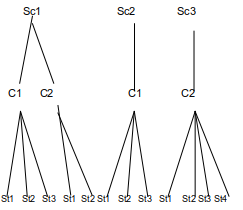
\includegraphics[width=0.4\linewidth]{screenshot001}
	\caption{Three-level models structure}
	\label{fig:screenshot001}
\end{figure}


\end{frame}

%
%\begin{frame}[shrink=5]
%\frametitle{\insertsection} 
%\framesubtitle{\insertsubsection}
%{\footnotesize
%	\begin{table}[]
%		\begin{tabular}{lllllll}
%			\hline
%			& \multicolumn{3}{l}{Classifications or levels} & GDP  & \multicolumn{2}{l}{Explanatory variables} \\ \hline
%			Date	& Industry $ i $	&  Region $ j $      &   Country $ k $     &  mln   & Continuous    &              Categorical        \\ \hline
%			2005 Q1		&   1    &     1  &     1 & 545  &   0.1        & 2         \\ \hline
%			2005 Q1		&    2   &      1 &    1  &  243 &   0.03        &  2        \\ \hline
%			2005 Q1		&     1  &   2    &   1   & 453 &        0.07
%			&1          \\ \hline
%			...		&    ...  &   ...   &  ...    & ... & ...          &       ...   \\ \hline
%		\end{tabular}
%	\end{table}
%}
%Continuous variables: Inflation, Unemployment
%
%Categorical variables: Development
%
%\end{frame}
%
%

%
%\begin{frame}[shrink=5]
%\frametitle{\insertsection} 
%\framesubtitle{\insertsubsection}
%
%Algebraic specification of random intercepts model:
%\begin{gather*}
%y_{ijk} = \beta_{0ijk} + \beta_1 x_{ijk} \\
%\beta_{0ijk} = \beta_0 + v_{0k} + u_{0jk} + e_{ijk}
%\end{gather*}
%
%
%$ i,j,k $ -  level 1,2,3 
%
%$ v_{0k}  $ - is the random effect at the country level, an allowed-to-vary departure from the grand mean; 
%$  u_{0jk} $ - is the random effect at the region level, a departure from the country effect; 
%$  e_{0ijk} $ - is the random effect at the industry level, a departure from the country  effect    within a region
%
%
%
%Random effects at different levels assumed to be uncorrelated
%
%
%
%\end{frame}
%

%\begin{frame}[shrink=5]
%\frametitle{\insertsection} 
%\framesubtitle{\insertsubsection}
%
%\begin{gather*}
%\rho_1 = \dfrac{\sigma^2_{v0}}{\sigma^2_{v0} + \sigma^2_{u0}}+ \sigma^2_{e}  \\ \rho_2 = \dfrac{\sigma^2_{v0} + \sigma^2_{u0} }{\sigma^2_{v0} + \sigma^2_{u0}}+ \sigma^2_{e}  
%\end{gather*}
%
%
%$ \sigma^2_{v_{0k}} $ - variance between countries; 
%$  \sigma^2_{u_{0jk}}    $ - variance between regions within countries;
%$  \sigma^2_{e_{ijk}}    $  - variance between industries within regions within countries;
%$ \sigma^2_{v_{0k}}   \sigma^2_{u_{0jk}}    $ - variance between regions 
%  
%Key notion is that highest level residual is a random, allowed-to-vary departure from general relationship
%
%Each lower level residual is allowed-to-vary random departure from the higher-level departure
%
%
%\end{frame}
%
%

%
%\begin{frame}[shrink=5]
%\frametitle{\insertsection} 
%\framesubtitle{\insertsubsection}
%
%\begin{figure}
%	\centering
%	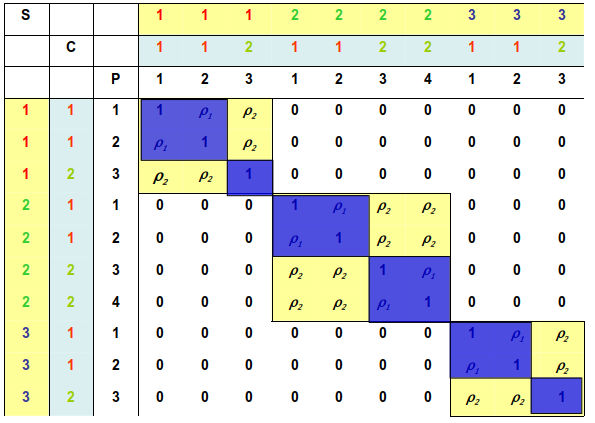
\includegraphics[width=0.7\linewidth]{screenshot002}
%	\caption{Correlation structure of 
%		3  level model: $ \rho_1 $ - intra-industry correlation (within same region \& country), $ \rho_2 $ - intra-region correlation (within same region, different industries)  }
%	\label{fig:screenshot002}
%\end{figure}
%
%
%\end{frame}
%

%\begin{frame}[shrink=5]
%\frametitle{\insertsection} 
%\framesubtitle{\insertsubsection}
%
%
%
%
%	\hfil\hfil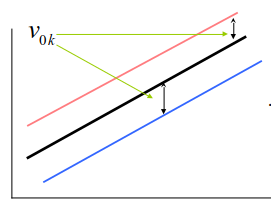
\includegraphics[width=5cm]{screenshot003}\newline
%	\null\hfil\hfil\makebox[5cm]{Level 3 residuals}\newline
%	\vfil
%	\hfil\hfil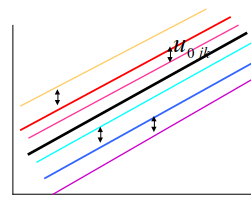
\includegraphics[width=5cm]{screenshot004}\hfil\hfil
%	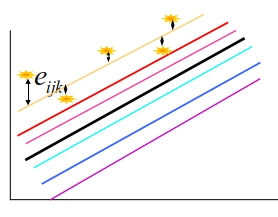
\includegraphics[width=5cm]{screenshot005}\newline
%	\null\hfil\hfil\makebox[5cm]{Level 2 residuals}
%	\hfil\hfil\makebox[5cm]{Level 1 residuals}
%
%
%\end{frame}
%
%



\subsection{Choosing datasets:} 


\begin{frame}[shrink=5]
\frametitle{\insertsection} 
\framesubtitle{\insertsubsection}

Данные:

\begin{itemize}
	\item для  eu:
	
	\begin{itemize}
		\item 3-уровневая: eu28 по странам по a10 (+)
		\item 2-уровневая: ввп по каждой из стран по a10 (?)
		\item 2 уровневая: eu28 стран по ввп 28 стран (+)
	\end{itemize}
	
	\item для rus:
	
	\begin{itemize}
		\item 3 уровневая: ввп по врп+налоги и прочее по отраслям (-) 
		\item 2 уровневая: только по врп (-)
		\item 2 уровневая: только по отраслям (произведенный по оквэд) (+)
		\item 2 уровневая: только по использованию (+)
		
	\end{itemize}
	
	\item для us:
	
	\begin{itemize}
		\item 3 уровневая: ввп по штатам и отраслям (?)
		\item 2 уровневая: ввп по штатам (+)
	\end{itemize}
		
\end{itemize}

\end{frame}



\subsection{US:} 

\begin{frame}[shrink=5]
\frametitle{\insertsection} 
\framesubtitle{\insertsubsection}

"Real Gross Domestic Product by Industry":

Квартальные данные с 2005-01-01 - 2018-04-01 по 50 штатам 

Millions of Chained 2012 Dollars 

Seasonally Adjusted Annual Rate:  

\begin{figure}
	\centering
	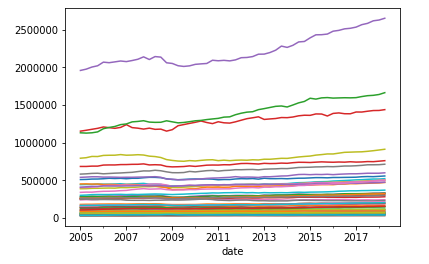
\includegraphics[width=0.7\linewidth]{screenshot007}
	\caption{Real Gross Domestic Product by State}
	\label{fig:screenshot007}
\end{figure}


\end{frame}


\begin{frame}[shrink=5]
\frametitle{\insertsection} 
\framesubtitle{\insertsubsection}

Разница между ВВП США и суммой ВДС для каждого штата (не больше 2\% ):


\begin{figure}
	\centering
	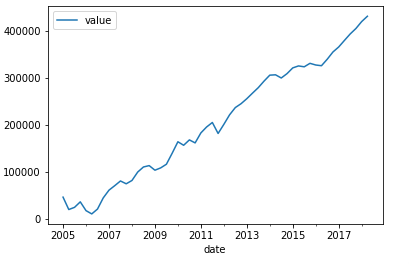
\includegraphics[width=0.7\linewidth]{screenshot013}
	\caption{Difference between GDP and sum of GVA by states:}
	\label{fig:screenshot013}
\end{figure}

\end{frame}




\subsection{Для России:} 


\begin{frame}[shrink=5]
\frametitle{\insertsection} 
\framesubtitle{\insertsubsection}


Данные по ВPП (в текущих ценах): 

для 79 регионов и 3 городов раз в год с 1995, 


\begin{figure}
	\centering
	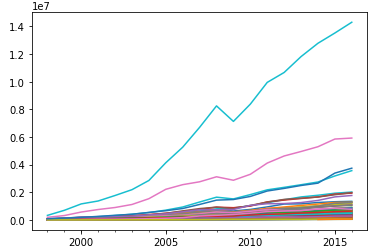
\includegraphics[width=0.7\linewidth]{screenshot014}
	\caption{ВРП по регионам}
	\label{fig:screenshot014}
\end{figure}


\end{frame}


\begin{frame}[shrink=5]
\frametitle{\insertsection} 
\framesubtitle{\insertsubsection}

Данные (в процентах от ВРП) для 79 регионов и каждой из 12 отраслей: 

%по 15 отраслям для каждого из 81 регионов (-4 автономные области) с 2004 по 2016 год  + "Деятельность домашних хозяйств"  c 2011 
%
%(1275  временных рядов по 12 наблюдений + 81 ряд по 5 наблюдений)
%

%GDP data by 15 sectors for each  of  85 regions, published once a year since 2004 (by region since 1995). 
%1275  time series total with 12 observations at least. 




\begin{figure}
	\centering
	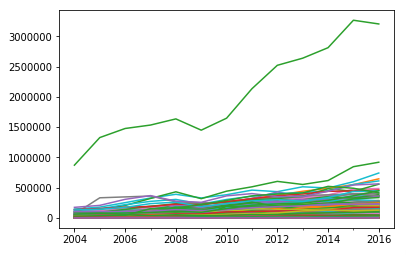
\includegraphics[width=0.7\linewidth]{screenshot015}
	\caption{ВРП по регионам по отраслям}
	\label{fig:screenshot015}
\end{figure}



\end{frame}




\begin{frame}[shrink=5]
\frametitle{\insertsection} 
\framesubtitle{\insertsubsection}

	\hfil\hfil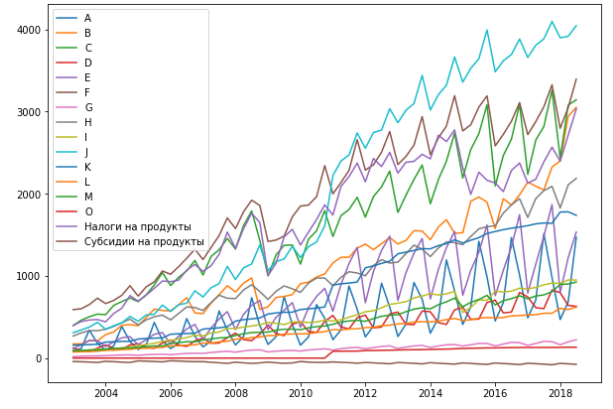
\includegraphics[width=5cm]{screenshot016}\newline
	\null\hfil\hfil\makebox[5cm]{ВВП квартальный (производственный метод):}\newline
	\vfil
	\hfil\hfil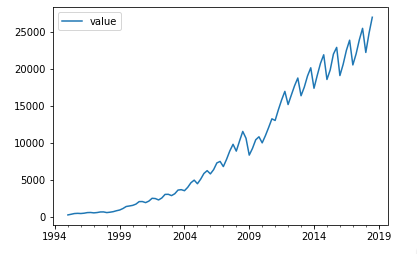
\includegraphics[width=5cm]{screenshot017}\hfil\hfil
	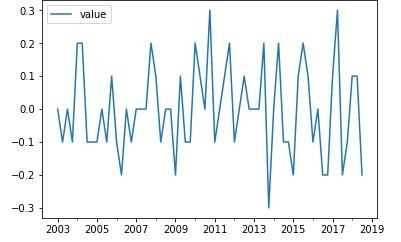
\includegraphics[width=5cm]{screenshot018}\newline
	\null\hfil\hfil\makebox[5cm]{ВВП квартальный}
	\hfil\hfil\makebox[5cm]{Разница (не более 0.00006 \%)}


\end{frame}



\begin{frame}[shrink=5]
\frametitle{\insertsection} 
\framesubtitle{\insertsubsection}




	\hfil\hfil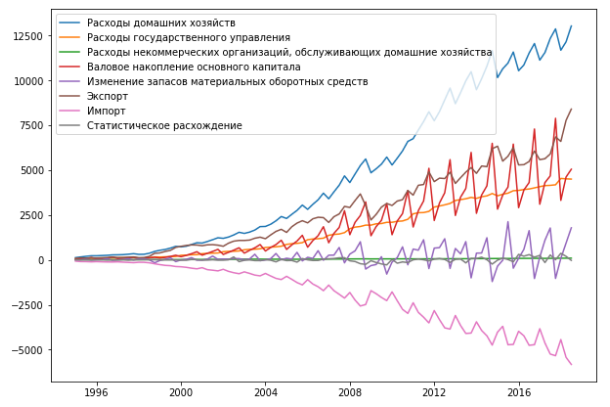
\includegraphics[width=5cm]{screenshot019}\newline
\null\hfil\hfil\makebox[5cm]{ВВП квартальный (по расходам): }\newline
\vfil
\hfil\hfil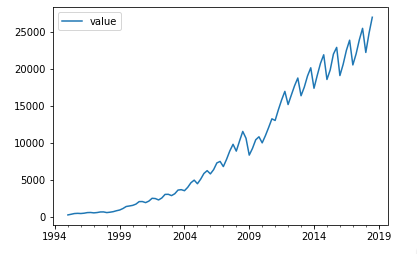
\includegraphics[width=5cm]{screenshot017}\hfil\hfil
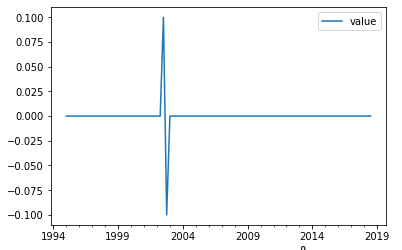
\includegraphics[width=5cm]{screenshot020}\newline
\null\hfil\hfil\makebox[5cm]{ВВП квартальный}
\hfil\hfil\makebox[5cm]{Разница (не более 0.00006 \%)}

\end{frame}




\subsection{ЕС:} 



\begin{frame}[shrink=5]
\frametitle{\insertsection} 
\framesubtitle{\insertsubsection}


Квартальные данные по ЕС по секторам: 

2000-01-01 по 2018-07-01


\begin{figure}
	\centering
	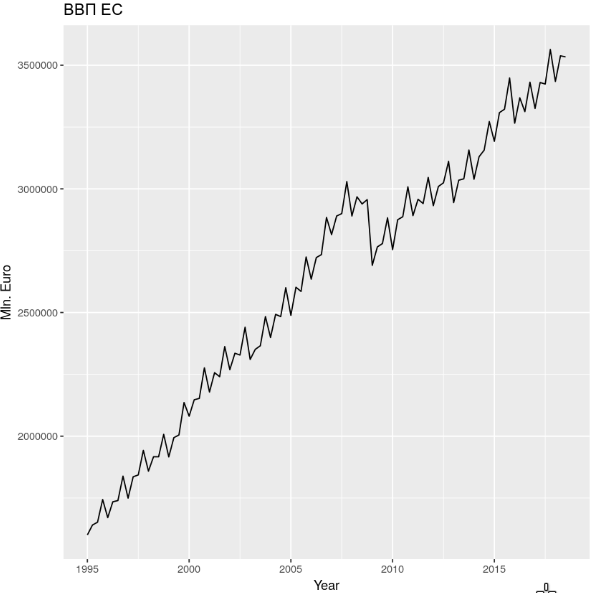
\includegraphics[width=0.7\linewidth]{screenshot021}
	\caption{ВВП ЕС28}
	\label{fig:screenshot021}
\end{figure}





\end{frame}


\section{Forecasting :} 

\subsection{Aggregated TS:} 


\begin{frame}[shrink=5]
\frametitle{\insertsection} 
\framesubtitle{\insertsubsection}



\begin{figure}
	\centering
	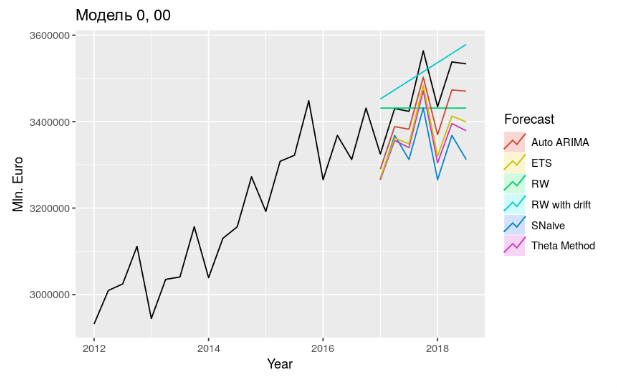
\includegraphics[width=0.7\linewidth]{screenshot022}
	\caption{Сравнение прогнозов}
	\label{fig:screenshot021}
\end{figure}





\end{frame}





\begin{frame}[shrink=5]
\frametitle{\insertsection} 
\framesubtitle{\insertsubsection}



\begin{figure}
	\centering
	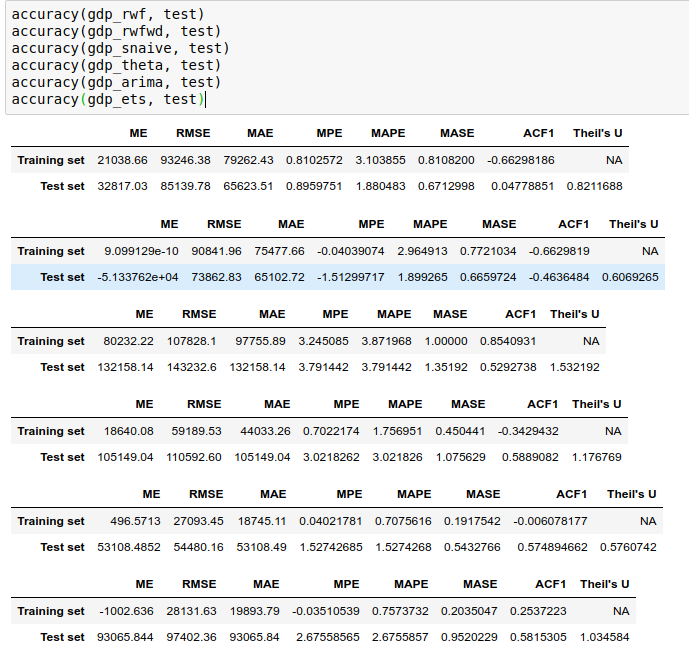
\includegraphics[width=0.7\linewidth]{screenshot023}
	\caption{Сравнение прогнозов}
	\label{fig:screenshot021}
\end{figure}





\end{frame}



\begin{frame}[shrink=5]
\frametitle{\insertsection} 
\framesubtitle{\insertsubsection}

\begin{figure}
	\centering
	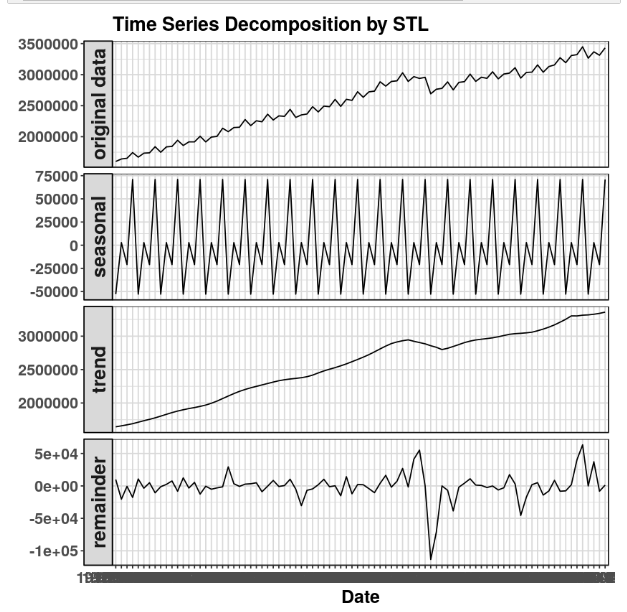
\includegraphics[width=0.7\linewidth]{screenshot024}
%	\caption{}
	\label{fig:screenshot024}
\end{figure}



\end{frame}



\begin{frame}[shrink=5]
\frametitle{\insertsection} 
\framesubtitle{\insertsubsection}

RPART, or CART (Classification and Regression Trees) is recursive partitioning type of binary tree for classification or regression tasks. It performs a search over all possible splits by maximizing an information measure of node impurity, selecting the covariate showing the best split.


\hfil\hfil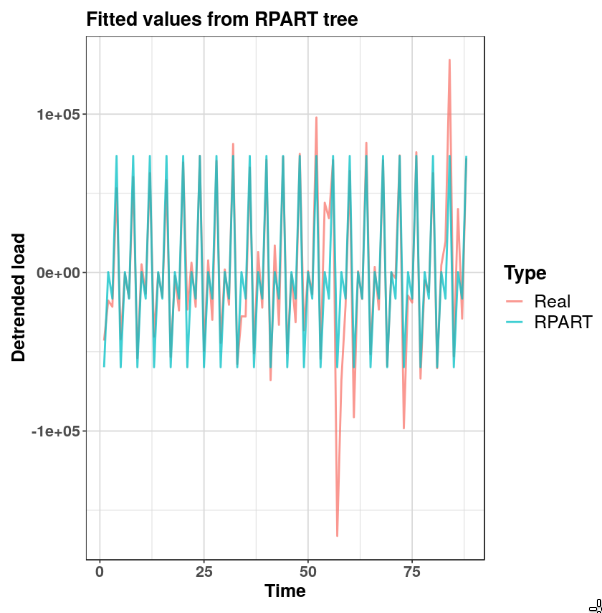
\includegraphics[width=5cm]{screenshot025}\hfil\hfil
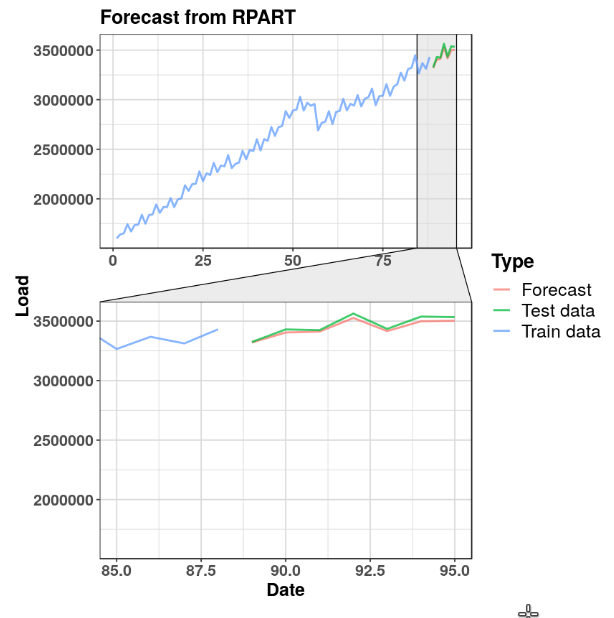
\includegraphics[width=5cm]{screenshot026}\newline
%\null\hfil\hfil\makebox[5cm]{Fit}
%\hfil\hfil\makebox[5cm]{Predict}


%
%\begin{figure}
%	\centering
%	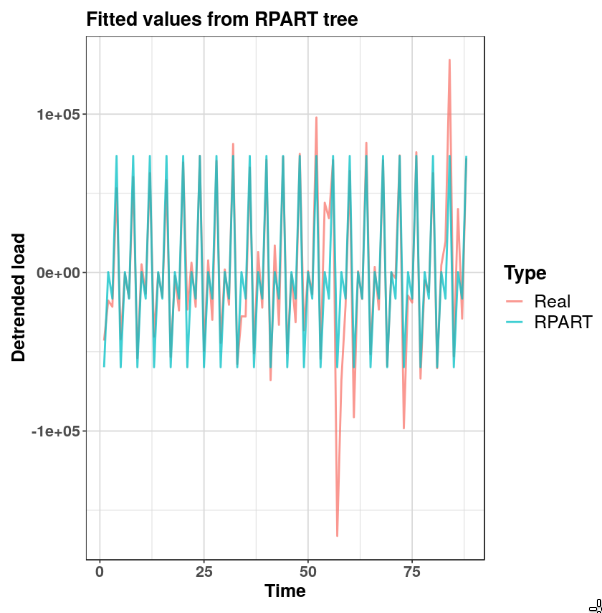
\includegraphics[width=0.7\linewidth]{screenshot025}
%	\caption{}
%	\label{fig:screenshot025}
%\end{figure}


\begin{figure}
	\centering
	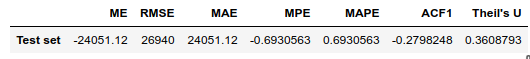
\includegraphics[width=0.7\linewidth]{screenshot027}
	\label{fig:screenshot027}
\end{figure}

\end{frame}



\subsection{Disaggregated TS}


\begin{frame}[shrink=5]
\frametitle{\insertsection} 
\framesubtitle{\insertsubsection}

\begin{figure}
	\centering
	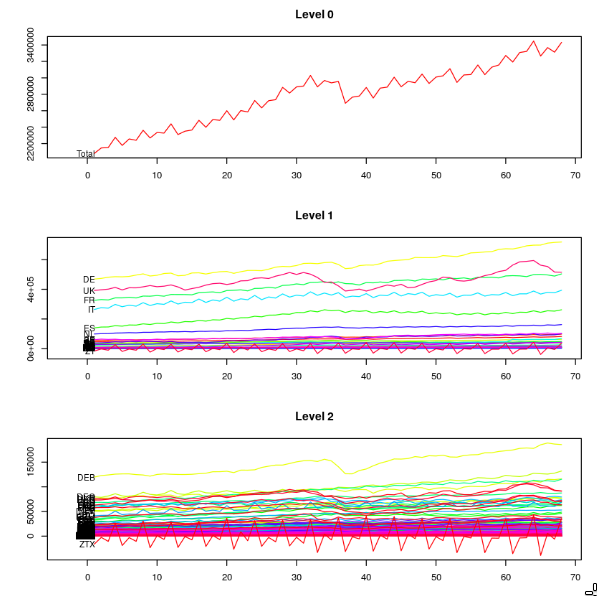
\includegraphics[width=0.7\linewidth]{screenshot028}
%	\caption{}
	\label{fig:screenshot028}
\end{figure}



\end{frame}



\section{Grouped Time Series}



\subsection{Forecasting hierarchical  time series}


\begin{frame}[shrink=5]
\frametitle{\insertsection} 
\framesubtitle{\insertsubsection}



The assumption upon which many of these models are built on, is that by grouping series that behave in a similar way, the idiosyncratic errors within groups will tend to offset each other while the more relevant individual dynamics will be retained to be modelled.



Key idea: forecast reconciliation
\begin{itemize}
	\item Ignore structural constraints and forecast
	every series of interest independently.
	\item Adjust forecasts to impose constraints.
\end{itemize}

Existing methods:
\begin{itemize}
	\item  Bottom-up
	\item  Top-down
	\item  Middle-out
	
\end{itemize}

An “optimal combination” 
approach can be advanced by proposing two new estimators
based on WLS.

Both now implemented in the hts package





\end{frame}


\begin{frame}[shrink=5]
\frametitle{\insertsection} 
\framesubtitle{\insertsubsection}

\begin{figure}
\centering
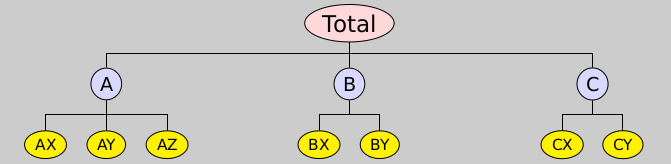
\includegraphics[width=0.7\linewidth]{screenshot010}
\caption{Hierarchical structure}
\label{fig:screenshot010}
\end{figure}


$ Y_t $ : observed aggregate of all
series at time $ t $.

$ Y_{ X , t} $ : observation on series X at
time t.

\end{frame}





\begin{frame}[shrink=5]
\frametitle{\insertsection} 
\framesubtitle{\insertsubsection}


For the hierarchical structure we can write: 

\[\begin{bmatrix}
y_{t} \\
y_{A, t} \\
y_{B, t} \\
y_{AA, t} \\
y_{AB, t} \\
y_{AC, t} \\
y_{BA, t} \\
y_{BB, t}
\end{bmatrix}
=
\begin{bmatrix}
1 & 1 & 1 & 1 & 1 \\
1 & 1 & 1 & 0 & 0 \\
0 & 0 & 0 & 1 & 1 \\
1  & 0  & 0  & 0  & 0  \\
0  & 1  & 0  & 0  & 0  \\
0  & 0  & 1  & 0  & 0  \\
0  & 0  & 0  & 1  & 0  \\
0  & 0  & 0  & 0  & 1
\end{bmatrix}
\begin{bmatrix}
y_{AA, t} \\
y_{AB, t} \\
y_{AC, t} \\
y_{BA, t} \\
y_{BB, t}
\end{bmatrix}\]


or in more compact notation,  where  $y_t$   is an $n$-dimensional vector of all the observations in the hierarchy at time $t$, $S$  is the summing matrix.

$$y_t  = S b_t$$


$ b_t $ : $m$-dimensional vector of all series at
bottom level in time t.


\end{frame}






\subsection{RW with drift}



\begin{frame}[shrink=5]
\frametitle{\insertsection} 
\framesubtitle{\insertsubsection}


\begin{figure}
	\centering
	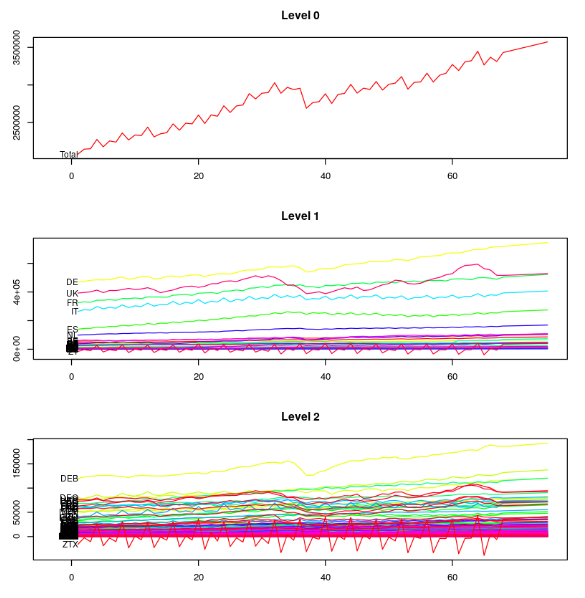
\includegraphics[width=0.7\linewidth]{screenshot029}
%	\caption{RW with drift}
	\label{fig:screenshot029}
\end{figure}


\end{frame}


\subsection{Snaive}


\begin{frame}[shrink=5]
\frametitle{\insertsection} 
\framesubtitle{\insertsubsection}


\begin{figure}
	\centering
	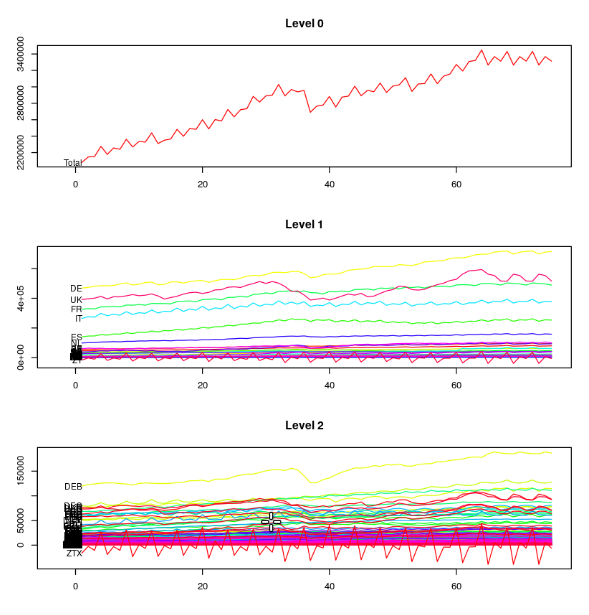
\includegraphics[width=0.7\linewidth]{screenshot032}
	%	\caption{RW with drift}
	\label{fig:screenshot029}
\end{figure}


\end{frame}


\subsection{Theta}


\begin{frame}[shrink=5]
\frametitle{\insertsection} 
\framesubtitle{\insertsubsection}

Equivalent to simple exponential smoothing with drift

\begin{figure}
	\centering
	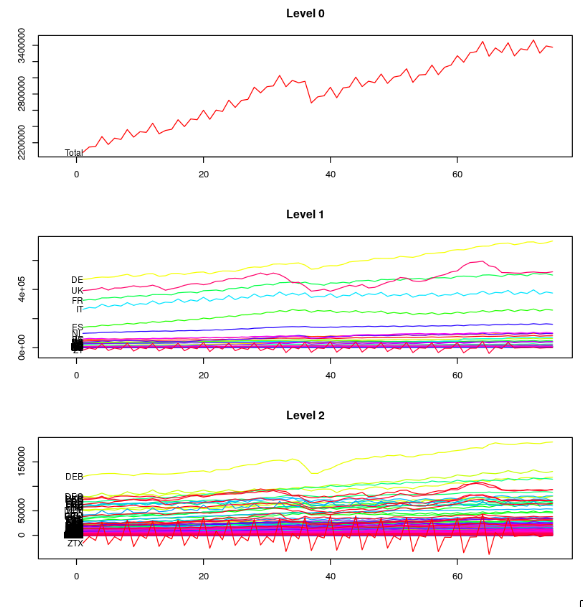
\includegraphics[width=0.7\linewidth]{screenshot034}
	%	\caption{RW with drift}
	\label{fig:screenshot029}
\end{figure}


\end{frame}

\subsection{ARIMA}


\begin{frame}[shrink=5]
\frametitle{\insertsection} 
\framesubtitle{\insertsubsection}


\begin{figure}
	\centering
	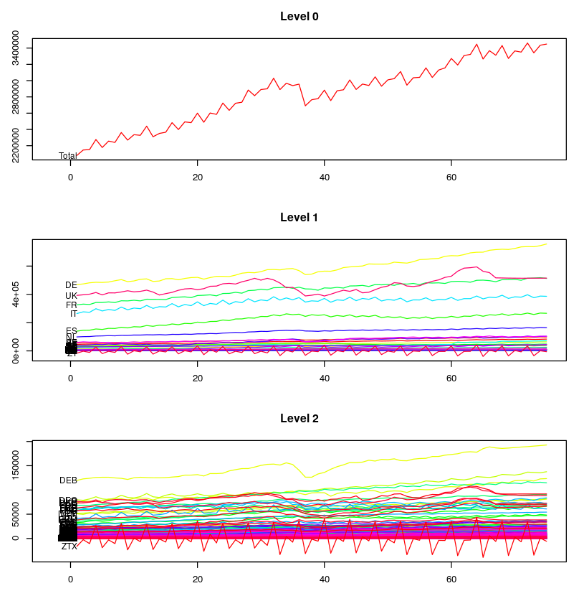
\includegraphics[width=0.7\linewidth]{screenshot037}
	%	\caption{RW with drift}
	\label{fig:screenshot029}
\end{figure}


\end{frame}




\begin{frame}[shrink=5]
\frametitle{\insertsection} 
%\framesubtitle{\insertsubsection}

%\begin{figure}
%	\centering
%	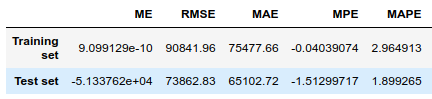
\includegraphics[width=0.7\linewidth]{screenshot031}
%	\caption{}
%	\label{fig:screenshot031}
%\end{figure}
%
%
%\begin{figure}
%	\centering
%	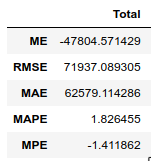
\includegraphics[width=0.7\linewidth]{screenshot030}
%	\caption{}
%	\label{fig:screenshot030}
%\end{figure}

\hfil\hfil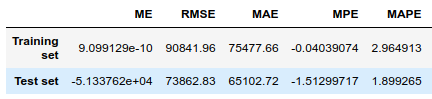
\includegraphics[width=5cm]{screenshot031}\hfil\hfil
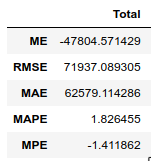
\includegraphics[width=1.5cm]{screenshot030}\newline


\hfil\hfil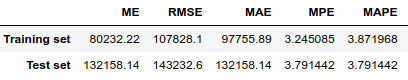
\includegraphics[width=5cm]{screenshot039}\hfil\hfil
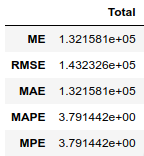
\includegraphics[width=1.5cm]{screenshot033}\newline

\hfil\hfil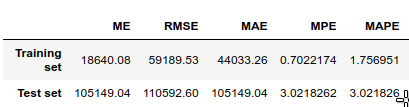
\includegraphics[width=5cm]{screenshot040}\hfil\hfil
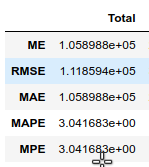
\includegraphics[width=1.5cm]{screenshot035}\newline


\hfil\hfil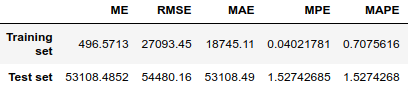
\includegraphics[width=5cm]{screenshot041}\hfil\hfil
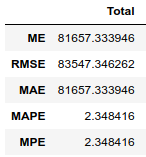
\includegraphics[width=1.5cm]{screenshot036}\newline


\end{frame}




\subsection{ARIMAX}


\begin{frame}[shrink=5]
\frametitle{\insertsection} 
\framesubtitle{\insertsubsection}


\begin{figure}
	\centering
	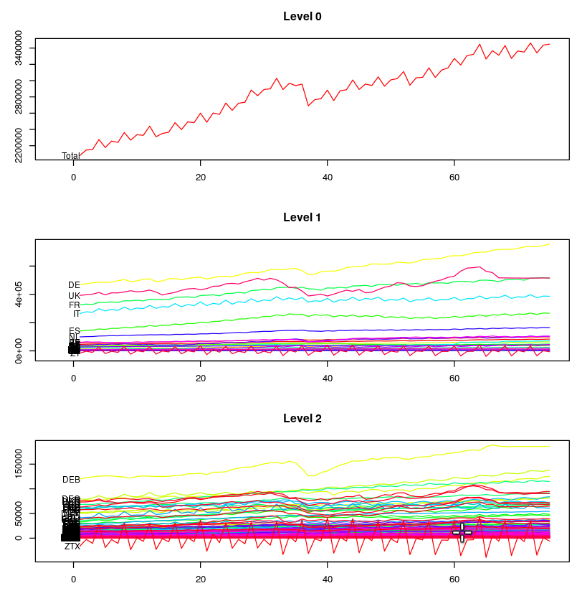
\includegraphics[width=0.7\linewidth]{screenshot038}
	%	\caption{RW with drift}
	\label{fig:screenshot029}
\end{figure}


\end{frame}


\begin{frame}[shrink=5]
\frametitle{\insertsection} 
\framesubtitle{\insertsubsection}


%\framesubtitle{\insertsubsection}

%\begin{figure}
%	\centering
%	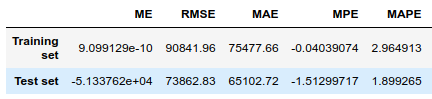
\includegraphics[width=0.7\linewidth]{screenshot031}
%	\caption{}
%	\label{fig:screenshot031}
%\end{figure}
%
%
%\begin{figure}
%	\centering
%	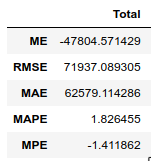
\includegraphics[width=0.7\linewidth]{screenshot030}
%	\caption{}
%	\label{fig:screenshot030}
%\end{figure}

\hfil\hfil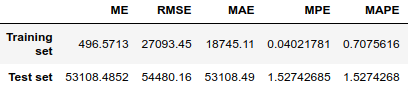
\includegraphics[width=5cm]{screenshot041}\hfil\hfil
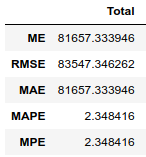
\includegraphics[width=1.5cm]{screenshot036}\hfil\hfil
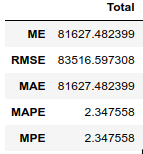
\includegraphics[width=1.5cm]{screenshot042}\newline


\end{frame}







\subsection{Forecasting 	grouped time series}


%
%\begin{frame}[shrink=5]
%\frametitle{\insertsection} 
%\framesubtitle{\insertsubsection}
%
%
%
%
%\[\begin{bmatrix}
%y_{t} \\
%y_{A, t} \\
%y_{B, t} \\
%y_{X, t} \\
%y_{Y, t} \\
%y_{AA, t} \\
%y_{AB, t} \\
%y_{AC, t} \\
%y_{BA, t} \\
%y_{BB, t}
%\end{bmatrix}
%=
%\begin{bmatrix}
%1 & 1 & 1 & 1 & 1 \\
%1 & 1 & 1 & 0 & 0 \\
%0 & 0 & 0 & 1 & 1 \\
%1 & 0 & 1 & 0 & 1 \\
%0 & 1 & 0 & 1 & 0 \\
%1  & 0  & 0  & 0  & 0  \\
%0  & 1  & 0  & 0  & 0  \\
%0  & 0  & 1  & 0  & 0  \\
%0  & 0  & 0  & 1  & 0  \\
%0  & 0  & 0  & 0  & 1
%\end{bmatrix}
%\begin{bmatrix}
%y_{AA, t} \\
%y_{AB, t} \\
%y_{AC, t} \\
%y_{BA, t} \\
%y_{BB, t}
%\end{bmatrix}\]
%
%
%\begin{figure}
%	\centering
%	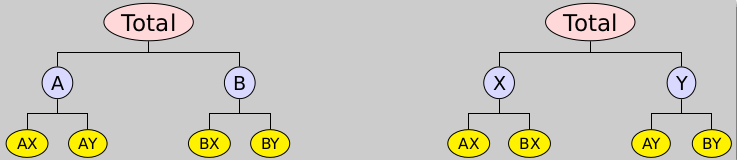
\includegraphics[width=0.7\linewidth]{screenshot011}
%	\caption{Grouped structure}
%	\label{fig:screenshot011}
%\end{figure}
%
%
%\end{frame}
%
%


%
%\subsection{Optimal forecasts}
%
%\begin{frame}[shrink=5]
%\frametitle{\insertsection} 
%\framesubtitle{\insertsubsection}
%
%\[ \hat{Y}_n ( h ) = S \beta_n ( h ) + e_h  \]
%
%$ \hat{Y}_n ( h ) $ - a vector of initial $ h $-step forecasts,
%made at time $ n $, stacked in same order as $ Y_t  $.
%
%$ \beta_n ( h )   = E [ B _{n + h} | Y_1 , \dots , Y_n ]  $
%
%$ e_h  $  has zero mean and covariance $ \Sigma_h  $.
%
%\[ \tilde{Y}_n ( h )
%= S \hat{\beta}_n ( h ) = S P  \hat{Y}_n ( h ) =  S ( S' \Sigma^{+}_h S )^{-1}  S'  \Sigma^{+}_h  \hat{Y}_n ( h )
% \]
% 
%$ \tilde{Y}_n ( h ) $   - revised forecasts, 
%$ \hat{Y}_n ( h ) $ - initial forecasts
%
%$ \Sigma^{+}_h $ - generalized inverse of $ \Sigma_h $.
%
%Optimal $ P = ( S' \Sigma^{+}_h S )^{-1}  S'  \Sigma^{+}_h  $
%
%Problem: $ \Sigma_h $ hard to estimate.
%
%\end{frame}
%

%
%\subsection{Approximate optimal forecasts}
%
%
%
%\begin{frame}[shrink=5]
%\frametitle{\insertsection} 
%\framesubtitle{\insertsubsection}
%
%
%\[ \tilde{Y}_n ( h )
%= 
% S ( S' \Sigma^{+}_h S )^{-1}  S'  \Sigma^{+}_h  \hat{Y}_n ( h )
%\]
%
%
%\begin{itemize}
%	\item OLS
%	
% 	 $ e_{B , h} $ is the forecast
%	error at bottom level.
%	
%	Assume $ e_h \approx S e_{B , h} $ 	
%	then $ ( S' \Sigma^{+}  S )^{-1} S'  \Sigma^{+} = ( S'S )^{ - 1} S'  $
%	
%	
%\[  \tilde{Y}_n ( h )
% =  S ( S'  S )^{-1}  S'   \hat{Y}_n ( h )
% \]	
%	
%	
%	\item Rescaling
%	
%	Suppose we approximate $ \Sigma_h $ by its diagonal: 
%$ \Lambda = diag(\hat{\Sigma}_1)^{-1}
% $,  which	
% contain inverse
%	one-step ahead in-sample forecast error
%	variances.
%	
%	\[ \tilde{Y}_n ( h )
%	=  S ( S'  \Lambda S )^{-1}  S'   \Lambda  \hat{Y}_n ( h )
%	\]
%	
%	\item Averaging
%	
%	If the bottom level error series are
%	approximately uncorrelated and have similar
%	variances, then $ \Lambda $ is inversely proportional to
%	the number of series contributing to each
%	node: 
%	$ \Lambda = diag( S \times 1 )^{- 1}
% $ is  the inverse row sums of S
% 
%\end{itemize}
%
%
%
%
%\end{frame}
%


%
%\subsection{Temporal hierarchies}
%
%
%
%\begin{frame}[shrink=5]
%\frametitle{\insertsection} 
%\framesubtitle{\insertsubsection}
%
%
%\textbf{Basic idea:}
%
%Forecast series at each available
%frequency. Optimally combine forecasts within the
%same year.
%
%
%\end{frame}
%
%
%




\section{Clusterization methods}

\section{Forecast-error clustering}


\begin{frame}[shrink=5]
\frametitle{\insertsection} 
\framesubtitle{\insertsubsection}


\begin{figure}
	\centering
	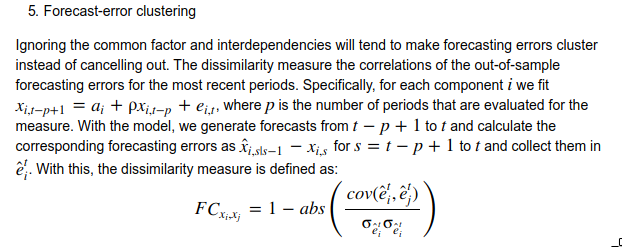
\includegraphics[width=0.7\linewidth]{screenshot043}
	%	\caption{RW with drift}
	\label{fig:screenshot029}
\end{figure}


\end{frame}



\section{The Diebold-Mariano Test}


\begin{frame}[shrink=5]
\frametitle{\insertsection} 
%\framesubtitle{\insertsubsection}


\begin{figure}
	\centering
	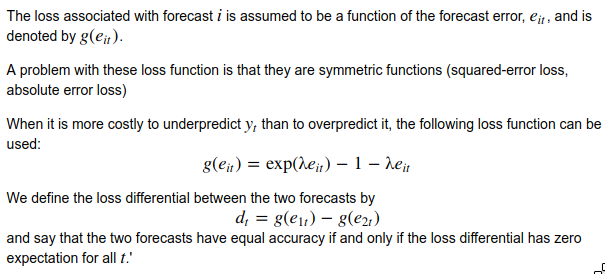
\includegraphics[width=0.7\linewidth]{screenshot044}
	%	\caption{RW with drift}
	\label{fig:screenshot029}
\end{figure}






\end{frame}


\begin{frame}[shrink=5]
\frametitle{\insertsection} 
%\framesubtitle{\insertsubsection}


\begin{figure}
	\centering
	\includegraphics[width=0.7\linewidth]{screenshot045}
	%	\caption{RW with drift}
	\label{fig:screenshot029}
\end{figure}






\end{frame}



\begin{frame}[shrink=5]
\frametitle{\insertsection} 
%\framesubtitle{\insertsubsection}


Harvey, Leybourne, and Newbold (1997) (HLN) suggest that
improved small-sample properties can be obtained by:
\begin{enumerate}
	\item  making a bias correction to the DM test statistic, and
\item  comparing the corrected statistic with a Student-t 
\end{enumerate}distribution with (T-1) degrees of freedom, rather than the standard normal.

$$HLN = DM\sqrt{(n+1-2h+h(h-1))/n} \sim T(n-1)$$

\begin{itemize}
	\item  The Diebold-Mariano test should not be applied
to situations where the competing forecasts are obtained using
two nested models, since  at the population level, if the
null hypothesis of equal predictive accuracy is true, the forecast errors from the competing models are exactly the same and perfectly correlated, which means that the numerator and denominator of a Diebold-Mariano test are each limiting to
zero as the estimation sample and prediction sample grow.

\item  However, when the size of the estimation sample remains finite, parameter
estimates are prevented from reaching their probability limits
and the Diebold-Mariano test remains asymptotically valid
even for nested models, under some regularity assumptions
(see Giacomini and White 2003).



\end{itemize}
\end{frame}



\section{Bayesian Methods}





\subsection{Why is the Bayesian Inference controversial?}

%\begin{frame}[shrink=5]
%\frametitle{\insertsection} 
%
%\textbf{Forward	modelling:	}   with
%  noise	
%properties	
%  we	
% can	 predict	
%  the	Sampling	
%  
%Distribution
%   (the probability	
%  for	
%  a	
% general	
%  set	
%  of	
% data
%
%
%In	
%  easy	
%  cases,	
%  the	
%  effect	
%  of	
%  the	
%  prior	
%  is	
%  simple. As	
%  experiment	
%  gathers	
%  more	
%  data,	
%  the	
%  likelihood	
%  tends	
%  to	
%  get	
%  narrower,	
%  and	
%  the	
%  influence	
%  of	
%  the	
%  prior	
%  diminishes.	
%  
%
%Rule	
%  of	
%  thumb:	
%  if	
%  changing	
%  your	
%  prior	
%  to	
%  another	
%  reasonable	
% one	
%  changes	
%  the	
%  answers	
%  significantly,	
%  you	
%  need	
%  more	
%  data	
%  
%
%
%
%\end{frame}
%
%


%
%\begin{frame}[shrink=5]
%\frametitle{\insertsection} 
%\framesubtitle{\insertsubsection}
%
%
%\begin{enumerate}
%	\item  Bayesians claim that the parameters are random so that their credible interval is a valid probability argument, though it also depends on the  the prior, which is usually hard to obtain.
%	
%	\item When the likelihood and prior is complicated, the inference has to rely on the MCMC sampling, which can be really slow in most of the real-world cases.
%
%	\item  The biggest controversy about Bayesian inference is that you must quantify your prior knowledge about the question at hand. This makes it possible to actually influence your results, either accidentally or on purpose. 	
%\end{enumerate}
%\end{frame}
%
%



%
%\subsection{Bayesian Modelling and Markov chain Monte Carlo}
%
%
%\begin{frame}[shrink=5]
%\frametitle{\insertsection} 
%\framesubtitle{\insertsubsection}
%
%Bayesian method provides an intuitive way for us to fill the gaps left by small or incomplete data sets. 
%
%
%To calculate the Bayesian predictive distribution, $\pi(x|D)$, given some data $D$,  we simply multiply the density function of the classical solution  $\ell (D|x)$,  with the density function produced by our prior knowledge $\pi(x)$. This is a direct application of Bayes’ theorem. Unfortunately, this product will not integrate to one. To overcome this, we multiply the density function by a constant $Z$, which rescales the density so that it does integrate to one. The resulting Bayesian distribution defined over the n-dimensional parameter space $S$ is
%
%$$ \pi(x|D) = \frac{1}{Z} \pi(x) \ell(D|x)$$
%
%$$ Z = \int_S \pi(x) \ell(D|x) dx$$
%
%In one dimension it is easy to use numerical quadrature to calculate $Z$. However as the dimension becomes large, this method quickly becomes impractical. So we turn to a class of statistical algorithms known as Markov chain Monte Carlo (MCMC) methods, which can tackle these high dimensional parameter spaces.
%
%
%
%\end{frame}
%
%
%


%\subsection{Bayesian Shrinkage}
%
%
%\begin{frame}[shrink=5]
%\frametitle{\insertsection} 
%\framesubtitle{\insertsubsection}
%
%\textbf{Shrinkage} is implicit in Bayesian inference and penalized likelihood inference, and explicit in James–Stein-type inference. In contrast, simple types of maximum-likelihood and least-squares estimation procedures do not include shrinkage effects, although they can be used within shrinkage estimation schemes.
% 
% 
% 
%\end{frame}

%\subsection{Stein's  paradox}
%
%
%\begin{frame}[shrink=5]
%\frametitle{\insertsection} 
%\framesubtitle{\insertsubsection}
% 
% 
%\textbf{Stein's  paradox}, in decision theory and estimation theory, is the phenomenon that when three or more parameters are estimated simultaneously, there exist combined estimators more accurate on average (that is, having lower expected mean squared error) than any method that handles the parameters separately. 
%
%\textit{The best guess about the future is usually  obtained by computing the average of past events. Stein's paradox defines circumstances in which there are estimators better that the arithmetic average
%}
%
%Stein’s paradox  **modern generalization, the Bayesian hierarchical model**. 
%
%Bayesian hierarchical model can improve overall estimation accuracy, thereby improving our confidence in the assessment results, especially for standard compliance assessment of waters with **small sample sizes.**
%
%
%\end{frame}
% 
\section{MCMC}
 
 
\section{Hierarchical Bayes}




\section{Small Sample}

%\begin{frame}[shrink=5]
%\frametitle{\insertsection} 
%
%
%Most of the inferential procedures available in the analysis of time series data are asymptotic
%
%Although analytic small sample results are available in a few cases, there is currently, no widely applicable and easily accessible method that can be used to make small sample inferences.
%
%\end{frame}
%


\section{Bootstrap}


%
%
%\begin{frame}[shrink=5]
%\frametitle{\insertsection} 
%
%
%The bootstrap technique introduced by Efron (1979) could possibly be a potential alternative in estimation and inference from time series models in finite samples. However, in time series regressions, the standard bootstrap resampling method designed for independent and identically distributed (IID) errors is not applicable because in most situations the assumption of IID errors is violated. 
%
%
%The basic bootstrap approach consists of drawing repeated samples (with replacement). 
%The simplest assumption for that method is that observations should be IID. 
%But in time series models IID assumption is not satisfied.
%Thus the method needs to be modified.
%
%	\begin{block}{BS for TS:}
%
%\begin{itemize}
%	\item Estimating Standard Errors:  if “Small Sample Size” distribution is normal then we can get a BS distribution to Estimate SE (same as asymptotic distribution for SE)
%	\item Confidence Interval statements:
%	Using BS distribution to Estimate CI we can get  different result for CI (from asymptotic distribution), for example, because of BS distribution skewness 
%\end{itemize}
%
%\end{block}
%
%\end{frame}
%
%

%
%\subsection{The Recursive BS for stationary AR(p) model}
%
%\begin{frame}[shrink=5]
%\frametitle{\insertsection} 
%\framesubtitle{\insertsubsection}
%
%
%Consider AR(p) process:
%\[ y_t = \sum_{i=1}^p a_i y_{t-i} + e_t, e_t \sim N(0,\sigma^2)\]
%
%We estimate coefficients with OLS and get: 
%\[ (\hat{a}_1,\dots, \hat{a}_p), \hat{e}_t \]
%
%
%
%
% Define the centered and scaled residuals:
%\[ \tilde{e}_t = (\hat{e}_{t} - \frac{1}{n} \sum \hat{e}_{t} )  \left( \frac{n}{n-p}\right) ^{1/2} \]
%Resample $ \tilde{e}_t $ with replacement to get the BS residuals $ e_t^* $
%
%Construct the BS sample recursively using $ y_t^* = y_t $:
%
%\[ y_t^* = \sum_{i=1}^p \hat{a}_i y_{t-i}^* + e_t^*\]
%
%
%\end{frame}
%
%
%\subsection{A comparison of four different block bootstrap methods}
%
%\begin{frame}[shrink=5]
%\frametitle{\insertsection} 
%\framesubtitle{\insertsubsection}
%
%
%
%
%\begin{figure}
%	\centering
%	\includegraphics[width=0.7\linewidth]{screenshot008}
%	\caption{MBB – Moving block bootstrap, 
%		NBB – Non-overlapping block bootstrap, 
%		SBB – Stationary block bootstrap, 
%		SS - Subsampling }
%	\label{fig:screenshot008}
%\end{figure}
%
%\end{frame}
%
%

%
%\subsection{Bootstrapping vs. Posterior sampling}
%
%\begin{frame}[shrink=5]
%\frametitle{\insertsection} 
%\framesubtitle{\insertsubsection}
%
%“Bootstrapping” is a a framework that aims to improve simple but approximate frequentist methods:
%
%\begin{itemize}
%	\item Parametric bootstrap: Improve asymptotic behavior of
%estimates for a trusted model: reduce bias of estimates,
%provide more accurate coverage of confidence regions
%
%\item Nonparametric bootstrap: Provide results that are
%approximately accurate with weak modeling assumptions
%
%\end{itemize}
%
%Most common approach uses Monte Carlo to simulate an ensemble
%of data sets related to the observed one, and use them to
%recalibrate a simple method.
%
%Parametric bootstrap has a step producing an ensemble of
%estimates that looks like a set of posterior samples. Can they be
%thought of this way?
%
%\end{frame}
%
%


\section{Maximum Entropy}




















\end{document}